%\renewcommand{\theequation}{\theenumi}
%\begin{enumerate}[label=\thesection.\arabic*.,ref=\thesection.\theenumi]
%\numberwithin{equation}{enumi}
\item  Find the centre and radius of the circle 
\begin{align}
x^2+y^2+8x+10y-8 = 0
\label{eq:circ_basic}
\end{align}
\solution
\eqref{eq:circ_basic} can be expressed as 
\begin{align}
\vec{x}^T\vec{x}+ 2\myvec{4 & 5}\vec{x} -8 = 0
\end{align}
which is of the form \eqref{eq:conic_quad_form} with
\begin{align}
\label{eq:circ_basic_uf}
\vec{u} = \myvec{4\\5}, f = -8
\end{align}
From  Table \ref{table:conics}, the center and radius are given by 
\begin{align}
\vec{c} = -\vec{u} = \myvec{-4\\-5},
r = \sqrt{\norm{u}^2-f} = 7
\end{align}
\item Find the equation of a circle which passes through the points $\vec{P} = \myvec{2\\-2}$ and $\vec{Q} = \myvec{3\\4}$ and whose centre lies on the line  
%\cite{eleven}
\begin{align}
\label{eq:circ_ex1_line}
\myvec{1 & 1} \vec{x} = 2
\end{align}
\solution From \eqref{eq:conic_quad_form} and Table \ref{table:conics}, the equation of a circle can be expressed as
\begin{align}
\label{eq:circ_conic}
\vec{x}^T\vec{x}-2\vec{c}^T\vec{x}+f = 0
\end{align}
where $\vec{c}$ is the centre.
Substituting the given points in 
\eqref{eq:circ_conic} and using 
\eqref{eq:circ_ex1_line}, the following equations are obtained
\begin{align}
2\myvec{2 & -2}\vec{c} -  f &= 8
\\
2\myvec{3 & 4}\vec{c} -  f &= 25
\\
\myvec{1 & 1}\vec{c}  &= 2
\end{align}
which can be expressed as the matrix equation
\begin{align}
\myvec{
1 & 1 & 0
\\
4 & -4 & -1 
\\ 
6 & 8 & -1  
}
\myvec{\vec{c}\\f} = \myvec{2\\8\\25}
\end{align}
Row reducing the augmented matrix
\begin{align}
\myvec{
1 & 1 & 0 & 2
\\
4 & -4 & -1 & 8
\\ 
6 & 8 & -1  & 25
}
\\
\xleftrightarrow[R_3 \leftarrow R_3 -6R_1]{R_2 \leftarrow -R_2+4R_1}
\myvec{
1 & 1 & 0 & 2
\\
0 & 8 & 1 & 0
\\ 
0 & 2 & -1  & 13
}
\\
\xleftrightarrow[R_3 \leftarrow -\frac{4R_3 -R_2}{2}]{R_1 \leftarrow 8R_1-R_3}
\myvec{
8 & 0 & -1 & 16
\\
0 & 8 & 1 & 0
\\ 
0 & 0 & 5  & -52
}
\\
\xleftrightarrow[R_2 \leftarrow \frac{5R_2 -R_3}{4}]{R_1 \leftarrow \frac{5R_1+R_3}{4}}
\myvec{
10 & 0 & 0 & 7
\\
0 & 10 & 0 & 13
\\ 
0 & 0 & 5  & -52
}
\end{align}
Thus, 
\begin{align}
\vec{c} &= \frac{1}{10}\myvec{7\\13}
\\
f &=-\frac{52}{5}
\end{align}
which give the desired equation of the circle.
From Table \ref{table:conics},
%
\begin{align}
 r =  \sqrt{\norm{\vec{c}}^2-f} = \frac{1}{10}\sqrt{1258}
\end{align}
Fig. \ref{fig:CircOr}	verifies the above results.

\begin{figure}[!ht]
\centering
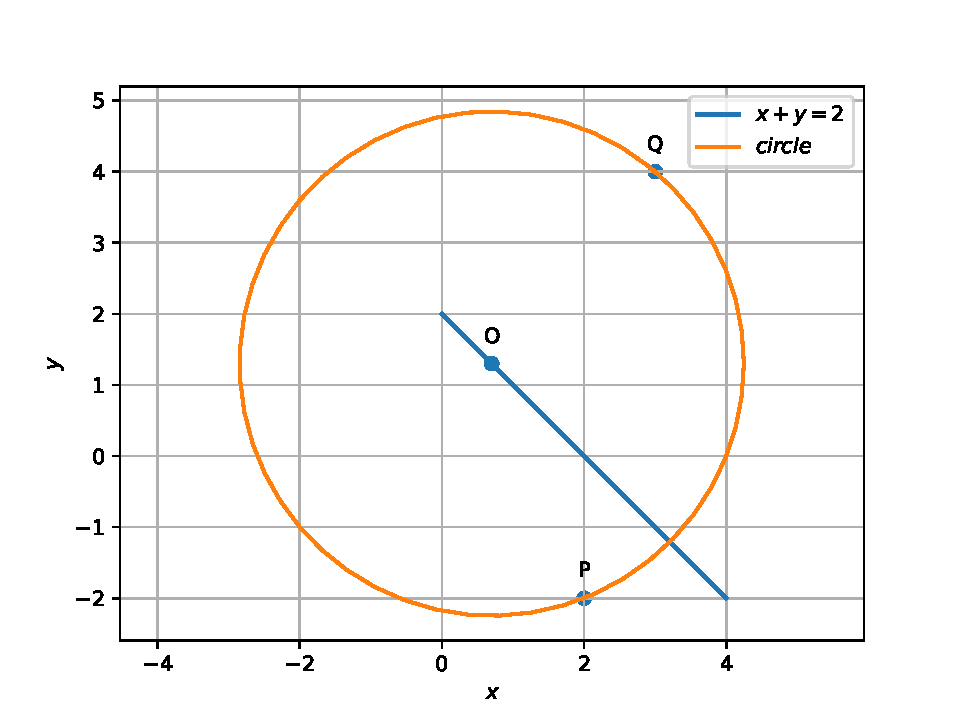
\includegraphics[width=\columnwidth]{./figs/circex/CircOr.eps}
\caption{Circle passing through $\myvec{2\\-2},\myvec{3\\4}$. Center is on line $\myvec{1 & 1}\vec{x}=2$. }
\label{fig:CircOr}	
\end{figure}

\item 
Find the points on the curve  
%\cite{twelve_one}
\begin{align}
x^2+y^2-2x-3 = 0
\label{eq:circle_tangent_prob}
\end{align}
at which the tangents are parallel to the $x$-axis.
\\
\solution \eqref{eq:circle_tangent_prob} can be expressed as
\begin{align}
\vec{x}^T\vec{x}+\myvec{-2 & 0}\vec{x}-3 &= 0
\label{eq:circle_tangent_prob_vec}
\\
\implies \vec{V} = \vec{I}, \vec{u} = \myvec{-1 \\ 0}, f = -3
\label{eq:circle_tangent_prob_uf}
\end{align}
From Table \ref{table:conics}, the centre and radius are
\begin{align}
\vec{c} = -\vec{u} = \myvec{-1 \\ 0}, r =\sqrt{\norm{\vec{u}}^2-f} = 2
\end{align}
$\because$ the tangents are parallel to the $x$-axis, their direction and normal vectors are respectively,
\begin{align}
\vec{m} = \myvec{1\\0},
\vec{n} = \myvec{0\\1}.
\end{align}
From Table \ref{table:conics},
\begin{align}
\kappa = \pm \sqrt{\frac{\vec{u}^T\vec{u}-f}{\vec{n}^T\vec{n}}} = \pm \sqrt{\frac{4}{1}} = \pm 2
\end{align}
and the desired points of contact are 
\begin{align}
\vec{q}_1, \vec{q}_2 = \myvec{1\\0}\pm 2\myvec{0\\1} =  
\myvec{1 \\  2},
\myvec{1 \\  -2}
\end{align}
%
Fig. \ref{fig:CircOr}	verifies the above results.
\begin{figure}[!ht]
\centering
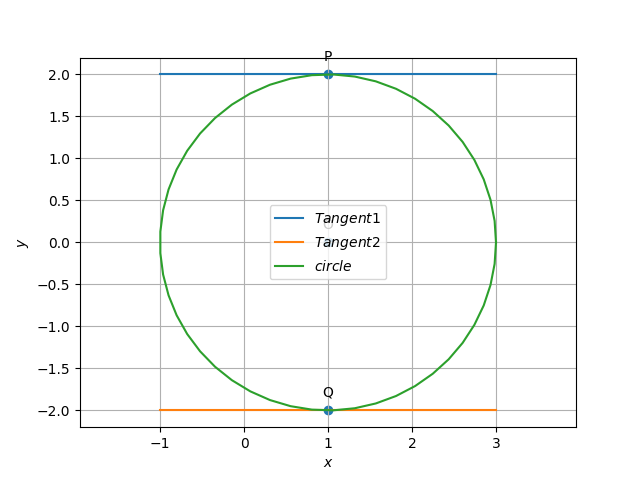
\includegraphics[width=\columnwidth]{./figs/circex/CircTangent.eps}
\caption{Tangents are parallel to the $x$-axis. }
\label{fig:CircTangent}	
\end{figure}

%\end{enumerate}
